\documentclass[class=article, crop=false]{standalone}
\begin{document}

\subsection{Posets}

A partially ordered set or \emph{poset} $(P, \leq)$ is a set $P$ with a relation $\leq$ on pairs in $P$ which encodes the topology of $\R$. The textbook \cite{gratzer_lattice_2011} provides a good introduction. An important note is that there is no requirement for every pair to be related, hence partial. We will use $P$ as shorthand for $(P, \leq)$ where possible.

In a poset $P$ we define the \emph{interval} between two elements $[x,y]$ as $[x,y] \coloneq \Set{u \in P \given x\leq u \leq y}$, which is itself a poset. A \emph{chain} is a subset $C \subseteq P$ that is a totally ordered, i.e~every pair in $(u,v) \in C\times C$ satisfies either $u\leq v$ or $v\leq u$. The \emph{covering relations} of $P$, denoted $\mathcal{E}(P)$ are defined,
\begin{equation*}
	\mathcal{E}(P) = \Set{(x,y) \in P\times P \given x\leq y \,\, \text{and} \,\,  [x,y] = \Set{x,y}}
\end{equation*}

i.e.~ordered pairs such that there is nothing in between them in the order. If $(x,y) \in \mathcal{E}(P)$, we write $x \lessdot y$. We will call a chain $C$ \emph{saturated} if for all $x,y \in C$ such that $x \leq y$, there exists $z \in C$ such that $x \lessdot z$, i.e.~there are no gaps in the chain.

By transitivity, the covering relations encode the whole poset structure, which can in turn be drawn in a diagram which we will now define.

\begin{definition}[Hasse Diagram]
	Given a poset $P$, the \emph{Hasse Diagram} is the directed graph encoding $\mathcal{E}(P)$ in the following way: For each element $x \in P$ draw a vertex. For each pair $(x,y) \in \mathcal{E}(P)$ draw an edge connecting $x$ to $y$.
\end{definition}

As is typical, we will draw the lesser (with respect to $\leq$) elements towards the bottom of the plane and visa versa. Thus, we will not need to draw arrows to show direction. The drawing of these Hasse diagrams is made easier as we will concern ourselves only with graded, bounded posets. \emph{Bounded} meaning that there are minimal and maximal elements, denoted $\hat{0}$ and $\hat{1}$ such that $\hat{0} \leq x \leq \hat{1}$ for all $x \in P$, and \emph{graded} meaning that every saturated chain from $\hat{0}$ to $\hat{1}$ has the same (finite) length. In the Hasse diagram for a bounded, graded poset, we will draw $\hat{0}$ at the bottom, $\hat{1}$ at the top, and put all other elements in discrete vertical levels between these based on the position in the saturated chains between $\hat{0}$ and $\hat{1}$ each element occurs. See \cref{fig:A4_interval} for an example.

\begin{figure}
	\centering
	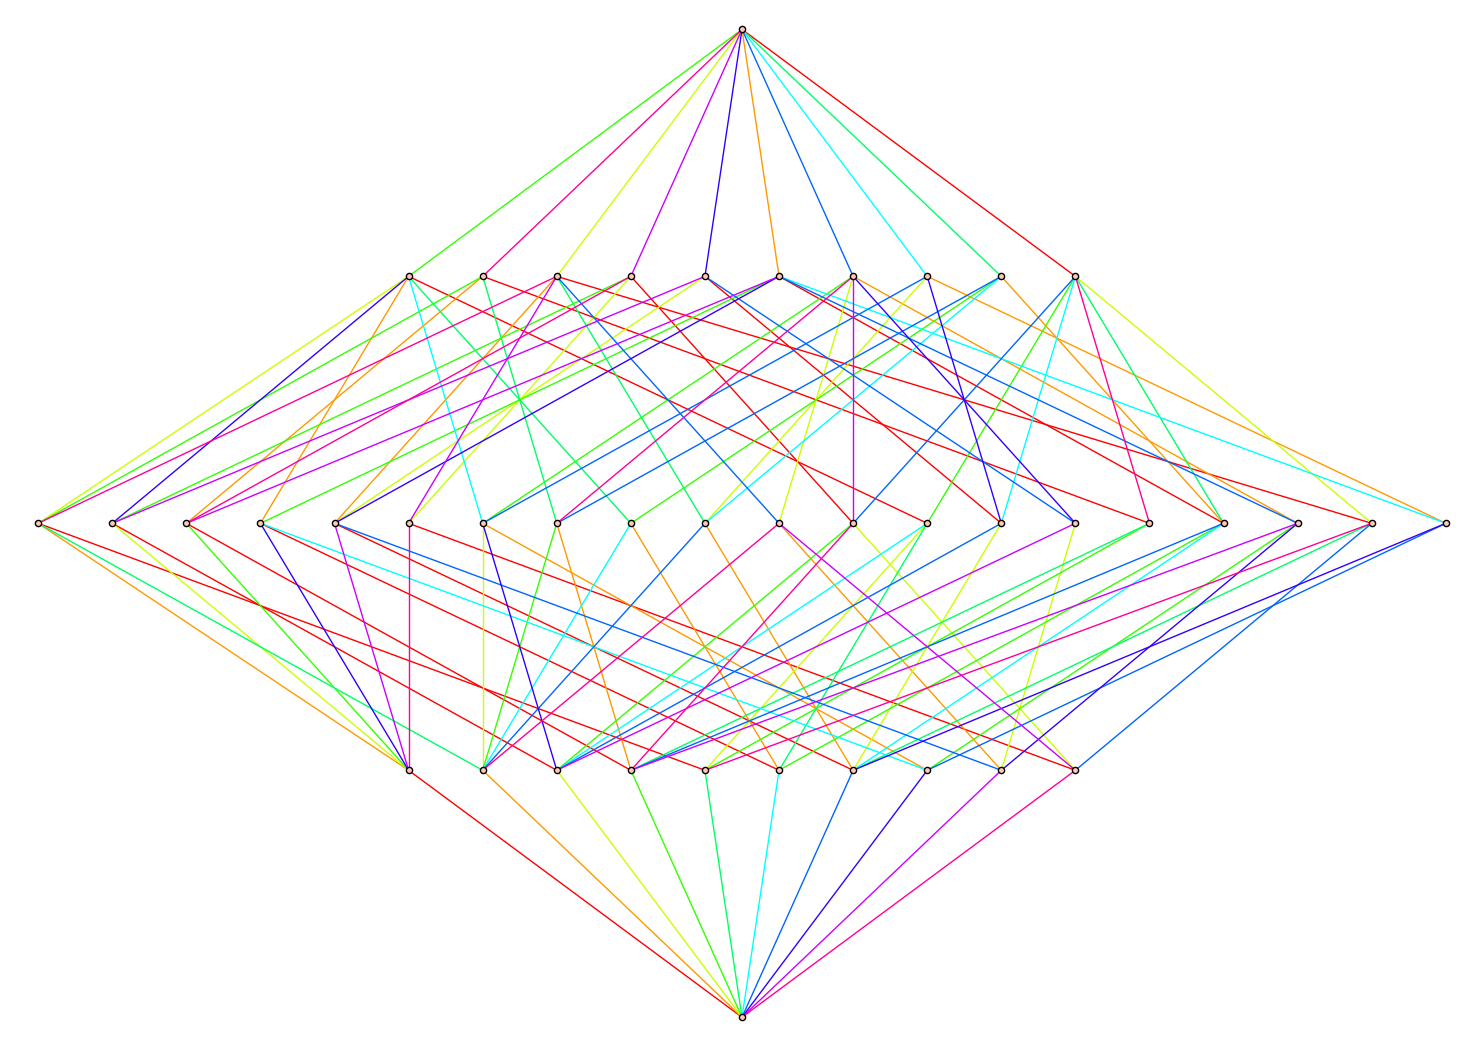
\includegraphics[width=7cm]{A4_interval.png}
	\caption{The poset $[1, abcd]^{A_4}$ as generated by all reflections, which label the edges by colour. An example of a bounded, graded, egde labelled poset. Generated using \texttt{Sage} and \texttt{GAP} \cite{sagemath_2020, gap_2022}}
	\label{fig:A4_interval}
\end{figure}

\begin{definition}[Edge Labelled Poset]
	We define an edge labelled poset to be a triple $(P,\leq,l)$ where $(P,\leq)$ is a poset and the function $l: \mathcal{E}(P) \to A$ is the data of our labels with $A$ being the alphabet of our labels.
\end{definition}

% filled small circle
\tikzstyle{FSC}=[circle,draw=black!50,fill=black!20,thick, inner sep=0pt,minimum size=1.5mm]
\tikzstyle{a}=[red]
\tikzstyle{b}=[blue]
\tikzstyle{c}=[black!30!green]
\tikzstyle{light}=[black!22!white]

\begin{figure}
\centering
\begin{tikzpicture}
	\node[FSC] (base)          	at (0,0)    						[label=below:$\emptyset$]         			{};
	\node[FSC] (bottom left)    at ($(base) + (-0.8,1) $)   		[label={[label distance=-0.1cm]200:$\{1\}$}]    {};
	\node[FSC] (bottom right)   at ($(bottom left) + (1.6,0)$)  	[label={[label distance=-0.1cm]300:$\{2\}$}]             		{};
	\node[FSC] (top left)       at ($(bottom left) + (-1.1,1)$)    	[label=left:{$\{1,2\}$}]          			{};
	\node[FSC] (top middle)    	at ($(base) + (0,2)$)  				[label=right:{$\{1,3\}$}]          			{};
	\node[FSC] (top right)    	at ($(bottom right) + (1.1,1)$)  	[label=right:{$\{2,3\}$}]          			{};
	\node[FSC] (top)          	at ($(base) + (0,3)$)    			[label=above:{$\{1,2,3\}$}]   				{};
	
	\draw[a] (base) 		to 	node[auto] 			{a} 	(bottom left);
	\draw[b] (base) 		to 	node[auto, swap] 	{b} 	(bottom right);
	\draw[b] (bottom left) 	to 	node[auto] 			{b} 	(top left);
	\draw[c] (bottom left) 	to 	node[auto] 			{c} 	(top middle);
	\draw[a] (top middle) 	to 	node[auto]			{a}		(top);
	\draw[a] (bottom right) to 	node[auto, swap] 	{a} 	(top right);
	\draw[a] (top left) 	to 	node[auto] 			{a} 	(top);
	\draw[b] (top right) 	to 	node[auto, swap] 	{b} 	(top);
\end{tikzpicture}
\hspace{1cm}
\begin{tikzpicture}[baseline=-18pt]
	\node[FSC] (base)          	at (0,0)    						    {};
	\node[FSC] (bottom left)    at ($(base) + (-0.8,1) $)   		    {};
	\node[FSC] (bottom right)   at ($(bottom left) + (1.6,0)$)  		{};
	\node[FSC] (top left)       at ($(bottom left) + (-1.1,0.5)$)    	    {};
	\node[FSC] (top middle)    	at ($(base) + (0,1.5)$)  				    {};
	\node[FSC] (top right)    	at ($(bottom right) + (1.1,0.5)$)  	    {};
	\node[FSC] (top)          	at ($(base) + (0,3)$)    			  	{};
	
	\draw (base) 			to 	 				(bottom left);
	\draw (base) 			to 	  				(bottom right);
	\draw (bottom left) 	to 	 				(top left);
	\draw (bottom left) 	to 	 				(top middle);
	\draw (top middle) 		to 					(top);
	\draw (bottom right) 	to 	  				(top right);
	\draw (top left) 		to 	 				(top);
	\draw (top right) 		to 	  				(top);
	
	
	\begin{pgfonlayer}{background}
		\draw[light] (base) 			to 	 				(top middle);
		\draw[light] (base) 			to 	  				(top);
		\draw[light] (base) 			to 	 				(top left);
		\draw[light] (base) 			to 	 				(top right);
		\draw[light] (bottom left) 	to 					(top);
		\draw[light] (bottom right) 	to 	  				(top);
	\end{pgfonlayer}
\end{tikzpicture}
\caption{A simple example of an edge labelled poset where we have taken $\leq$ to be $\subseteq$ (left). The same poset with all chains drawn in light lines to aid visualiseing $\Delta(P)$ (right).}
\label{fig:example_edge_labelled_poset}
\end{figure}

We will use $P$ as a shorthand for $(P,\leq,l)$ where possible. Given an edge labelled poset $P$, we can construct a group encoded by its labelling and geometry.

\begin{definition}[Poset group]
	\label{def:poset_group}
	Given some edge labelled poset $(P,\leq,l \colon \mathcal{E}(P) \to A)$, let the poset group $G(P)$ be the group generated by $\image(l)$ with relations equating words corresponding to saturated chains going up the Hasse diagram of $P$ which start and end at the same vertices.
\end{definition}

A \emph{word corresponding to a saturated chain} is the word of the labels traversed in the Hasse diagram while tracing out that saturated chain. In the example given in \cref{fig:example_edge_labelled_poset}, the poset group is $G(P) = \GroupPres{a,b,c \relations aba=bab,\, ba=ca}$.

\end{document}